%! Author = Adrian Helberg

% Preamble
\documentclass[12pt]{beamer}
% Theme
\usetheme{Boadilla}

% Bibliography
\bibliography{literature}
\bibliographystyle{plain}

% Packages
\usepackage{amsmath}
\usepackage[utf8]{inputenc}
\usepackage{ngerman}
\usepackage{graphicx}
\usepackage{color}
\usepackage{xcolor}
\usepackage[export]{adjustbox}
% Remove frame break numbering
\setbeamertemplate{frametitle continuation}{}

\subtitle{Template-basierte Synthese von\\Verzweigungsstrukturen mittels L-Systemen}
\title{Bachelorarbeit Kolloquium}
\author{Adrian Helberg}
\institute{HAW Hamburg}
\date{\today}
\titlegraphic{
\includegraphics[scale=0.25]{../images/HAW_Marke_CMYK.pdf}}

% Document
\begin{document}
    \frame{\titlepage}
    \frame{\frametitle{Agenda} \tableofcontents}

    \section{Einleitung}
    \label{sec:thema}
    \begin{frame}[allowframebreaks]
        \frametitle{Einleitung: Titel}

        \begin{block}{Titel}
            \color{olive}\underline{\color{black}Template-basierte} \color{teal}\underline{\color{black}Synthese} 
            \color{black}von \color{orange}\underline{\color{black}Verzweigungsstrukturen} \color{black}mittels 
            \color{cyan}\underline{\color{black}L-Systemen}
        \end{block}

        \begin{itemize}
            \item[\color{olive}$\rightarrow$] \color{black}Verschiedene Muster als kleinste zu organisierende Einheit
            \item[\color{teal}$\rightarrow$] \color{black}Verknüpfung von Verzweigungen zu einer neuen Struktur
            \item[\color{orange}$\rightarrow$] \color{black}Baumstrukturen als Ergebnis der Synthese
            \item[\color{cyan}$\rightarrow$] \color{black}Formale Grammatik zur Kodifizierung von Strukturen
        \end{itemize}
    \end{frame}

    \begin{frame}
        \frametitle{Einleitung: Relevanz}

        \begin{itemize}
            \setlength\itemsep{1em}
            \item Digitalisierung
            \item Kein einsteigerfreundliches Gebiet
            \item Automatisierte Erstellung von digitalen Inhalten
            \begin{itemize}
                \item "`Natürlichkeit der Dinge"'
            \end{itemize}
            \item Regeln und Muster kodifizieren
            \item Künstliche Intelligenz
        \end{itemize}
    \end{frame}

    \begin{frame}
        \frametitle{Einleitung: Ziele}

        \begin{block}{Zentrale Aufgabe}
            System zur Umsetzung einer Synthese von Strukturen, die einer Eingabestruktur ähneln
        \end{block}

        \begin{itemize}
            \setlength\itemsep{1.4em}
            \item Methodiken und Algorithmen aus der aktuellen Forschung
            \begin{itemize}
                \item Praktikabilität
                \item Anwendung am Beispiel eines Programms
            \end{itemize}
            \item Erzeugen von Ähnlichkeit
            \item Automatisierte Erstellung
        \end{itemize}
    \end{frame}

    \section{Forschung}
    \label{sec:forschung}
    \begin{frame}
        \frametitle{Forschung: Verwandte Arbeiten}
        
        \begin{figure}
            \centering
            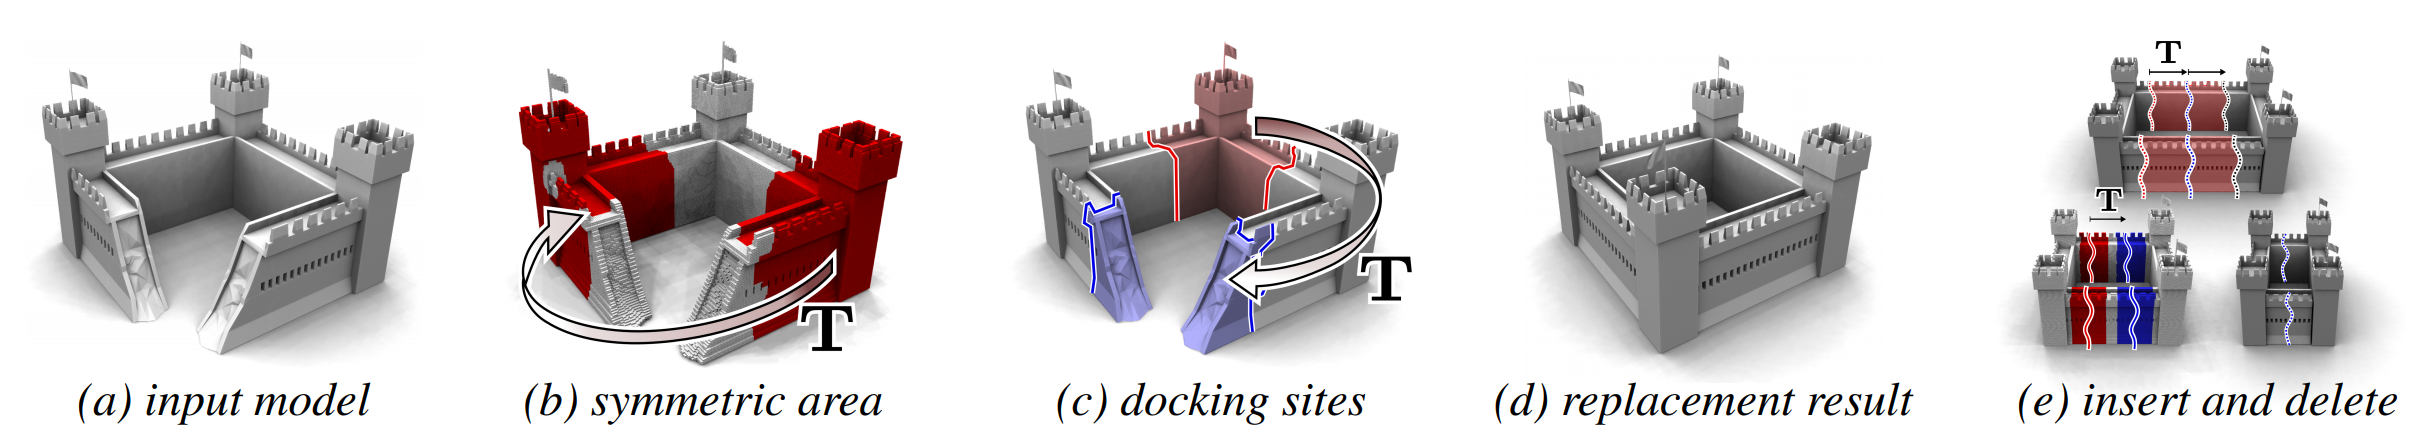
\includegraphics[width=12cm]{../images/bokeloh_2010_system.PNG}
            \caption{Textur- und Geometriesynthese anhand lokaler Ähnlichkeit}
        \end{figure}
    \end{frame}

    \begin{frame}
        \frametitle{Forschung: Verwandte Arbeiten}

        \begin{figure}
            \centering
            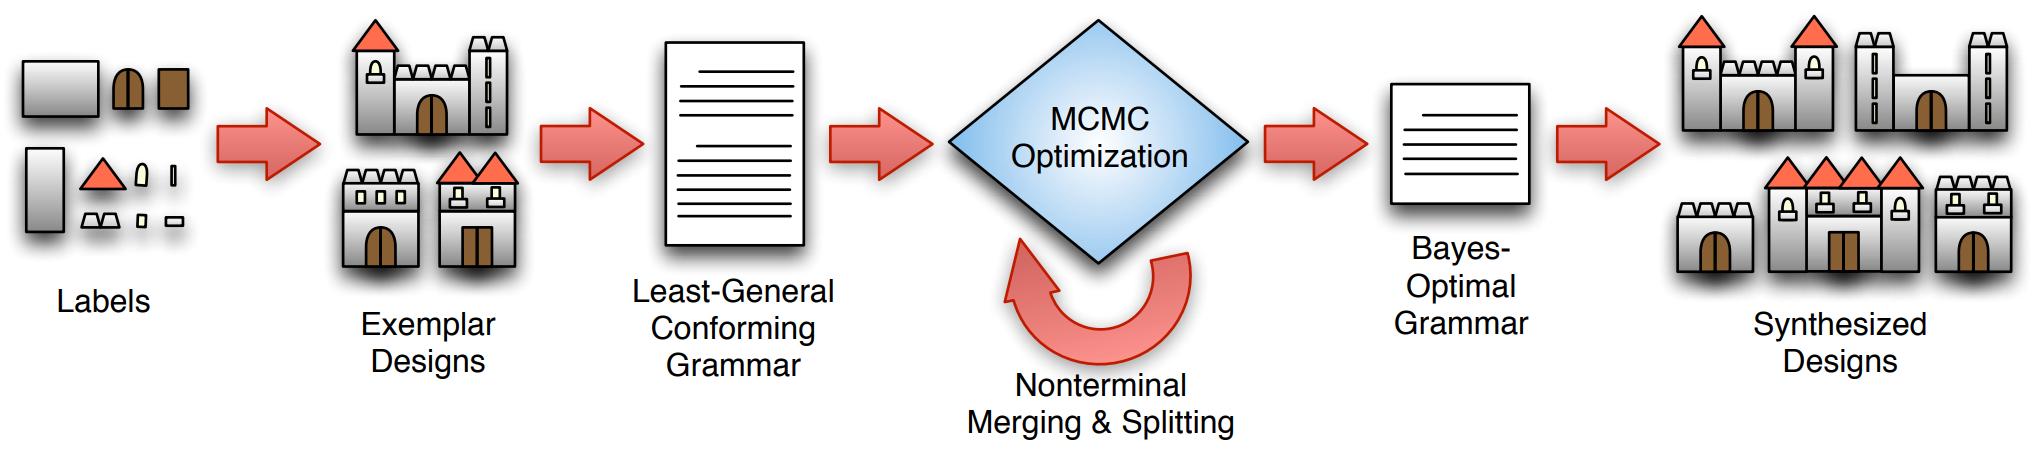
\includegraphics[width=12cm]{../images/talton_2012_system.PNG}
            \caption{Algorithmische Methode zum Lernen von Design Patterns}
        \end{figure}
    \end{frame}

    \begin{frame}
        \frametitle{Forschung: Verwandte Arbeiten}

        \begin{figure}
            \centering
            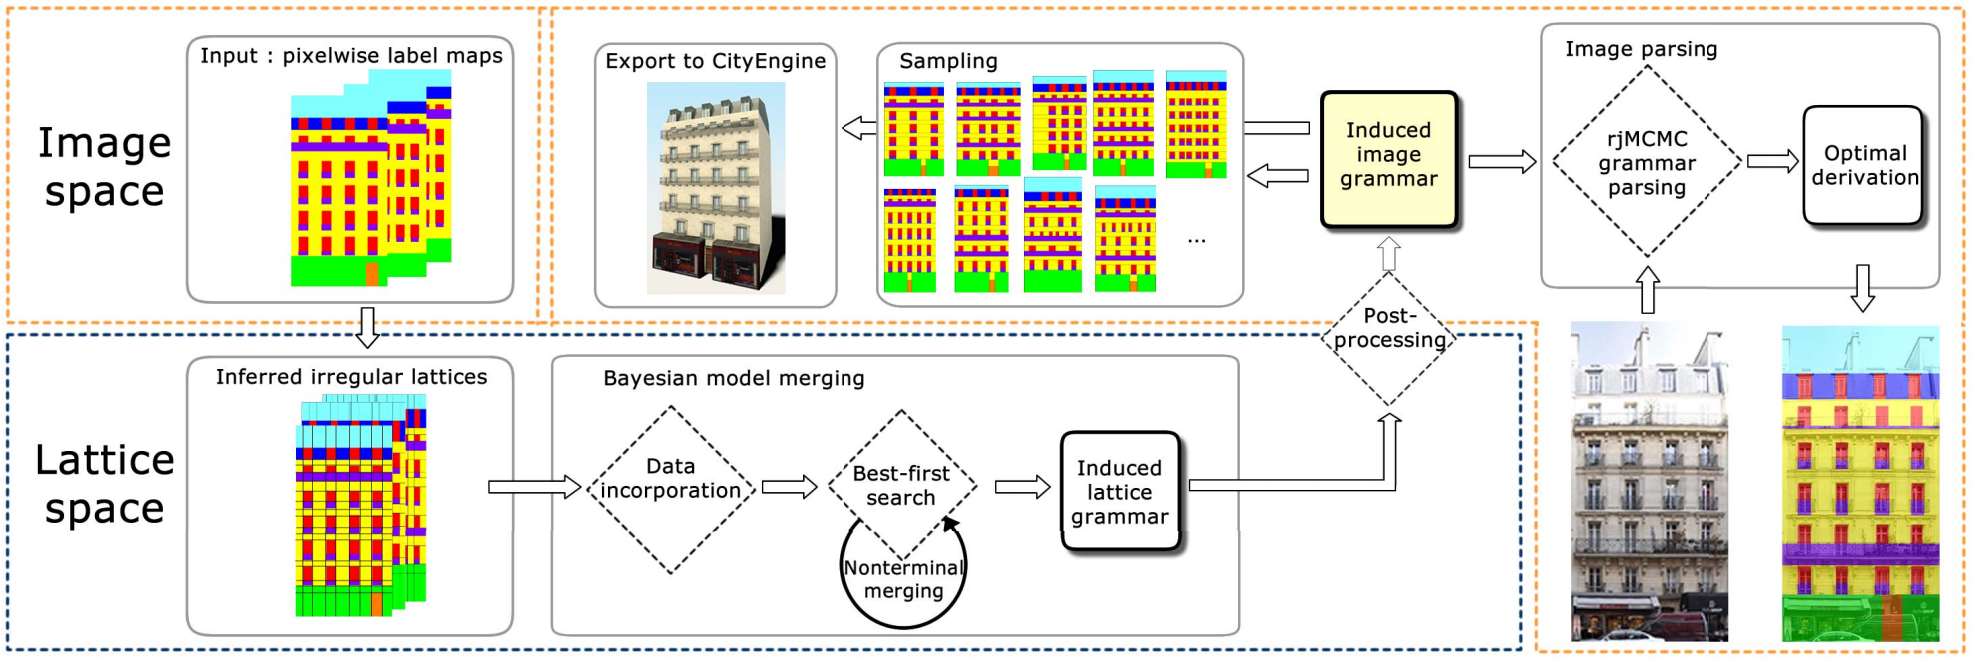
\includegraphics[width=12cm]{../images/martinovic_2013_system.PNG}
            \caption{Synthetisierung neuer Baustile und Rekonstruktion von Gebäuden}
        \end{figure}
    \end{frame}

    \begin{frame}
        \frametitle{Forschung: Verwandte Arbeiten}

        \begin{figure}
            \centering
            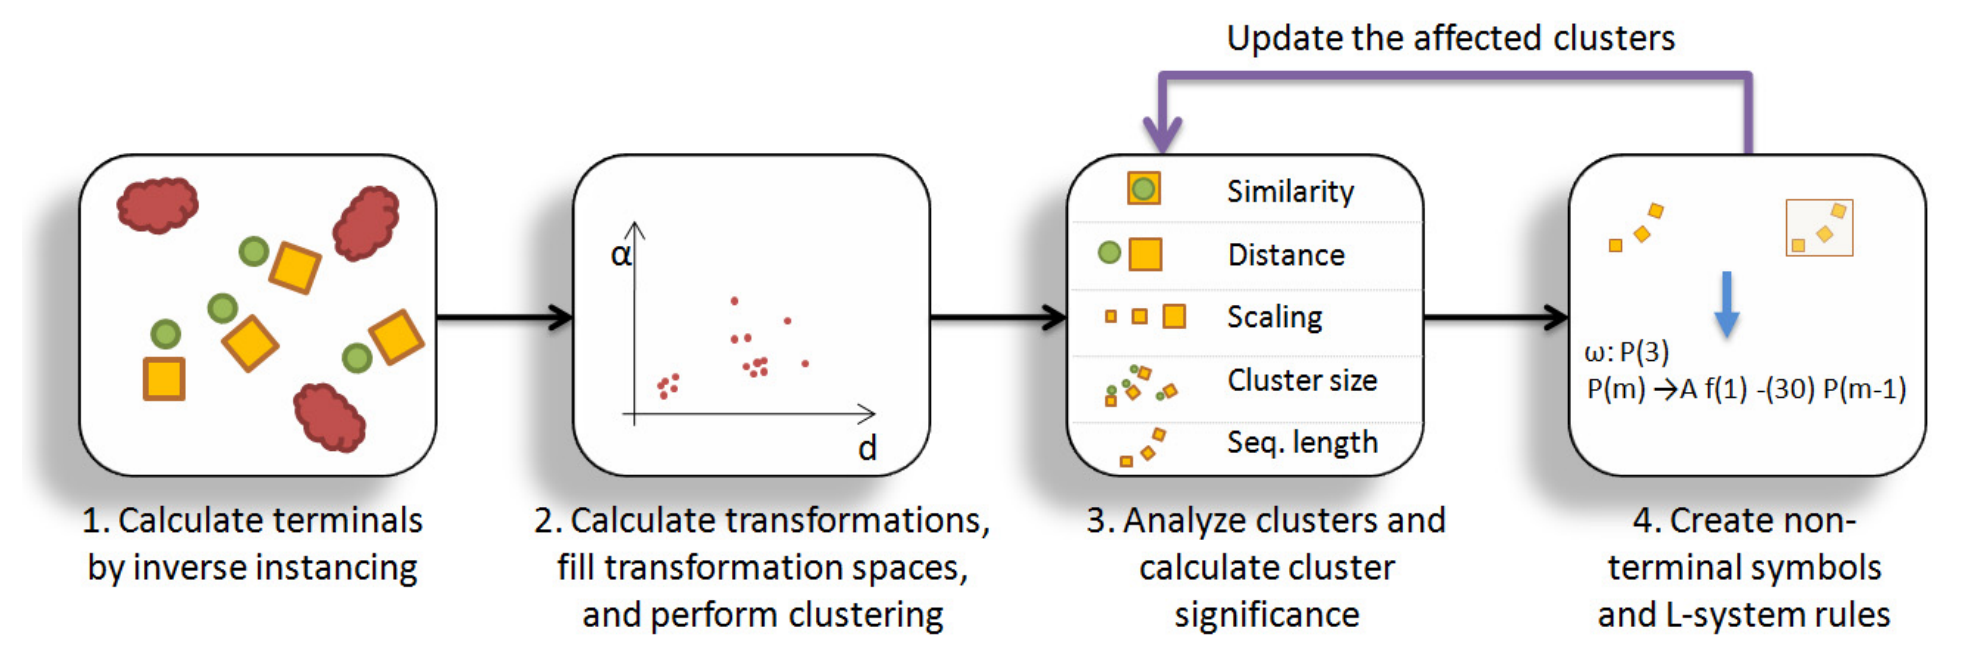
\includegraphics[width=12cm]{../images/stava_2010_system.PNG}
            \caption{System-Pipeline zur Erzeugung eines L-Systems eines 2D-Modells}
        \end{figure}
    \end{frame}

    \begin{frame}
        \frametitle{Forschung: Verwandte Arbeiten}

        \begin{figure}
            \centering
            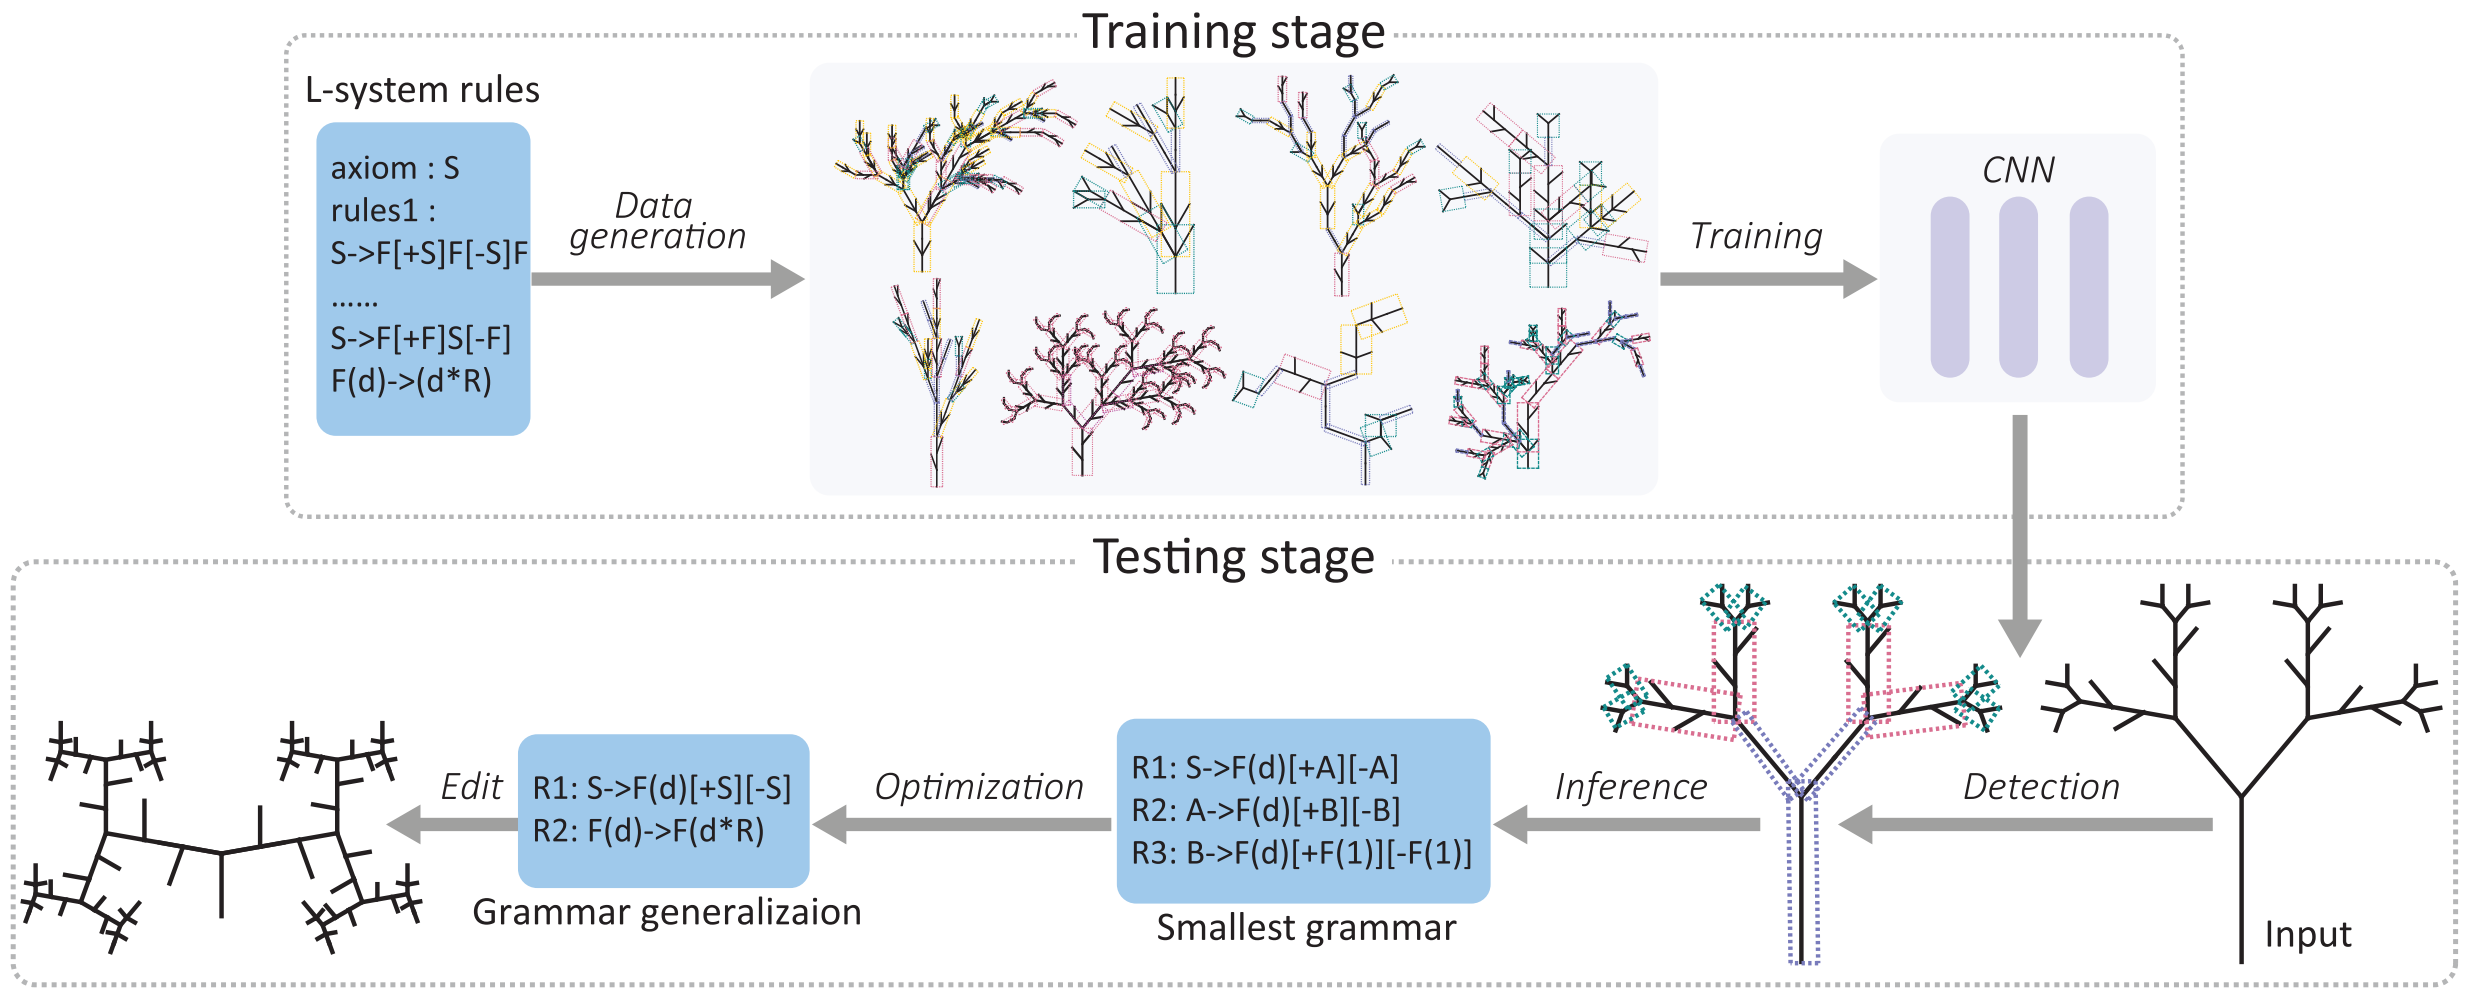
\includegraphics[width=12cm]{../images/guo_2020_system.PNG}
            \caption{Bearbeitung von L-System-Repreäsentationen zur Erzeugung von Ähnlichkeit}
        \end{figure}
    \end{frame}

    \section{Methodik}
    \label{sec:methodik}
    \begin{frame}
        \frametitle{Methodik}

        \begin{columns}
            \column{0.5\textwidth}
            \begin{itemize}
                \setlength\itemsep{1em}
                \item Strukturieren
                \item Datenaufbereitung
                \item Inferieren
                \item Komprimieren
                \item Generalisieren
            \end{itemize}

            \column{0.5\textwidth}
            \begin{itemize}
                \setlength\itemsep{1em}
                \item Visualisieren
                \item Randomisieren
            \end{itemize}
        \end{columns}
    \end{frame}

    \section{Ergebnisse}
    \label{sec:ergebnisse}
    \begin{frame}
        \frametitle{Ergebnisse}

        \begin{figure}
            \centering
            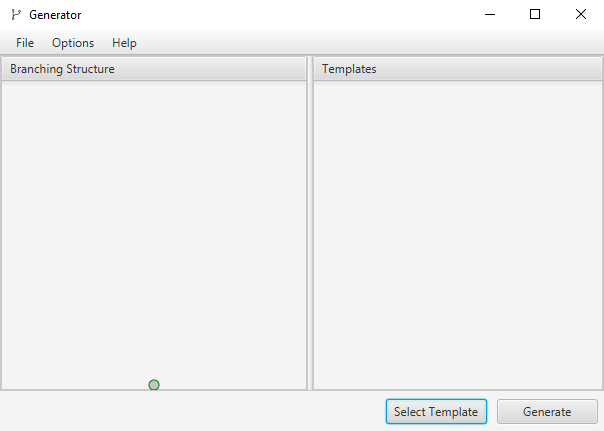
\includegraphics[width=8cm,cfbox=blue 0.4pt 1pt]{../images/UI.PNG}
            \caption{Umgesetztes Programm}
        \end{figure}
    \end{frame}

    \section{Fazit}
    \label{sec:fazit}
    \begin{frame}
        \frametitle{Fazit}
    \end{frame}

\end{document}